\documentclass{article} 
\usepackage{polski}
\usepackage[utf8]{inputenc} 
\usepackage[OT4]{fontenc} 
\usepackage{graphicx,color}
\usepackage{url} 
\usepackage[pdftex,hyperfootnotes=false,pdfborder={0 0 0}]{hyperref} 
\usepackage{indentfirst}
\usepackage{longtable}
\usepackage{multicol}

\title{Algorytmy izotermicznego sekwencjonowania przez hybrydyzację}
%\date{October 31, 2014}%
\author{ \\ Piotr Kurzawa (117245) \\ Marek Rydlewski (117214)}

\graphicspath{ {images/} }

\begin{document}

\maketitle

\vspace{3ex}

\tableofcontents

\newpage

\section{Wstęp}

Celem tego projektu było zaimplementowanie algorytmów izotermicznego sekwencjonowania przez hybrydyzację z błędami negatywnymi.

W klasycznym sekwencjonowaniu przez hybrydyzację wykorzystuje się bibliotekę oligonukleotydów o równej długości, a poszczególne jej elementy mają różną temperaturę topnienia. Utrudnia to takie dobranie warunków eksperymentu biochemicznego, aby wszystkie oligonukleotydy w danej temperaturze tworzyły stabilne dupleksy z analizowaną sekwencją, co ma wpływ na liczbę występujących błędów hybrydyzacji.

Izotermiczne SBH w przeciwieństwie do swojej wersji klasycznej nie wymaga używania wszystkich oligonukleotydów o wcześniej ustalonej długości. Podejście to wykorzystuje oligonukleotydy, w których stała jest nie długość, lecz parametr temperatury topnienia dla całego oligonukleotydu. 

W ISBH biblioteka izotermiczna składa się ze wszystkich oligonukleotydów o pewnej temperaturze T, na którą w danym dupleksie składają się sumy stopni wszystkich tworzących go par nukleotydów. Na podstawie późniejszych badań przyjęto, że sekwencję DNA zawsze można odtworzyć na podstawie spektrum otrzymanego przy wykorzystaniu dwóch bibliotek izotermicznych różniących się o temperaturą o 2 stopnie Celsjusza (pary nukleotydów A/T dodają 2 stopnie do łącznej temperatury topnienia dupleksu, natomiast pary C/G - 4 stopnie). W praktyce, podejście to okazuje się skuteczniejsze od klasycznego, szczególnie w przypadku występowania w spektrum błędów negatywnych.

Niniejsze sprawozdanie zawiera opis zaimplementowanych przez nas algorytmów (dokładnym i przybliżonym), przeprowadzone testy oraz wnioski będące jednocześnie porównaniem opracowanych rozwiązań problemu izotermicznego sekwencjonowania przez hybrydyzację.


%Błędy negatywne - ISBH izotermiczne sekwencjonowanie (jeden rodzaj błędu)%

%0, 1, {2, 3}, {4, 5}, wiele%

Oba algorytmy zostały zaimplementowane w języku C++11 i były testowane na platformach Windows (w środowisku Visual Studio 2015) oraz OS X (z użyciem kompilatora Apple LLVM/Clang w wersji 7.3.0). 

\section{Algorytm przybliżony}
\subsection{Ogólne założenia}
W rozwiązaniu przybliżonym zdecydowaliśmy się na skorzystanie z algorytmu ewolucyjnego, a konkretnie z algorytmu genetycznego. Ta heurstyka znana jest ze swojej skuteczności w rozwiązywaniu wielu problemów obliczeniowo trudnych. Zdecydowaliśmy się na taki algorytm również dlatego że posiadamy doświadczenie w dość skutecznej implementacji takich heurstyk oraz znaleźliśmy w literaturze fachowej wiele przykładów na jego efektywność właśnie w problematyce sekwencjowania DNA. Ogólna idea programu jest prosta - losowana jest pewna populacja początkowa, która poddawana jest selekcji (ocenie). Najlepsze osobniki biorą udział w reprodukcji - genotypy rodziców są krzyżowane, a na otrzymanym potomstwie przeprowadzana jest mutacja, która ma za zadanie zwiększyć różnorodność i wyjść z ewentualnego optimum lokalnego. Jako wejście algorytmu przyjmujemy mapę gdzie klucze to kolejne oligonukletody w postaci stringów a wartości to odpowiednie klasy, zaimplementowane w postaci typu wyliczeniowego.

\subsection{Opis algorytmu}
Nasz algorytm został zaprojektowany do radzenie sobie z błędami negatywnymi, ale krótkie eksperymenty pokazały że radzi sobie również z problematyką sekwencjowania z błędami obu rodzajów.

Algorytm tworzy spektrum oligonukleotydów wykorzystując wejściową mapę -  do spektrum zaliczamy górną granicę danej klasy - tym sposobem gwarantujemy że nie pominiemy żadnego oligo w naszym rozwiązaniu. Jak poradziliśmy sobie z błędami negatywnymi opiszemy później (w punkcie mutacje). 

W naszym algorytmie funkcja oceny polega na skonstruowaniu wynikowego DNA stosując maksymalny overlapping przyległych oligonukleotydów w wektorze. Im więcej oligonukleotydów uda nam się zmieścić nie przekraczając długości n - długości DNA tym lepsza ocena rozwiązania. Uważny czytelnik zauważy że początkowe rozwiązania mogą przekraczać długość n co w problemie sekwencjowania z błędami negatywnymi jest dość nietypowe, jednakże taka jest natura losowych początkowych rozwiązań. Warto zwrócić uwagę, ze bardzo szybko algorytm redukuje długość rozwiązania poniżej n. Aby nie pozwolić na zbytnie skrócenie rozwiązania, zwłaszcza przy większej ilości błędów w fazie mutacji stosujemy dodanie losowych oligonukleotydów w takiej sytuacji. Finalnym rozwiązaniem jest ciąg oligonukleotydów najlepszego osobnika.

\begin{enumerate}
\item Wylosowanie populacji początkowej
\begin{itemize}
\item Osobniki to obiekty klasy, zawierające w sobie m.in wektor liczb, który określa kolejność oligonukleotydów w rozwiązaniu - liczby wskazują na poszczególne indeksy tablicy zawierającej wszystkie oligonukleotydy wejściowe
\item Losowanie polega na permutacji w oparciu o liczby pseudolosowe wykorzystując generator Mersenn'a z ziarnem które jest prawdziwą liczbą losowa
\end{itemize}
\item Ocena i wybór najlepszych osobników
\begin{itemize}
\item Wybieramy najlepsze osobniki i kierujemy je do reprodukcji, odsetek premiowanych osobników wyznaczyliśmy eksperymentalnie.
\end{itemize}
\item Krzyżowanie - wybieramy losowe pary z najlepszych rodziców. Odsetek potomków wyznaczamy doświadczalnie.
\begin{itemize}
\item Kolejne oligonukleotydy dziecka dobieramy w myśl zasady:
\begin{enumerate}
\item Wyszukujemy oligonukleotyd w obu rodzicach
\item Oceniamy overlapping między tym oligonukleotydem a następnym oligo w rodzicu
\item Porównujemy i wybieramy oligonukleotyd o większym overlappingu, w przypadku remisu wyboru dokonujemy losowo. Fakt wybrania oligo zaznaczamy w tablicy oligonukleotodyów już zużytych.
\item Jeśli oligonukleotyd nie ma następnika, lub następnik został już użyty wyszykujemy inny niewykorzystany jeszcze oligonukleotyd rodzica o jak największym overlappingu.
\end{enumerate}
\item Jak widać zastosowaliśmy tutaj krzyżowanie wielopunktowe
\end{itemize}
\item Mutacje - aby uniknąć wpadnięcia w lokalne optimum i zwiększyć przeszukiwaną przestrzeń rozwiązań stosujemy mutacje trzech rodzajów
\begin{itemize}
\item Wyszukujemy oligonukleotyd który ma najmniejszy overlapping z obu stron tj. za równo ze strony następnika jak i poprzednika. Następnie zamieniamy miejscami ten oligonukleotyd z sąsiadem - to czy zamienimy go z następnikiem czy poprzednikiem zależy który ma mniejszy swój sumaryczny overlapping (wybieramy tego gorszego). Zastosowanie takich mutacji pozwala na eliminację potencjalnych "słabych podciągów" w rozwiązaniu
\item Wybieramy dwa oligonukletody i zamieniamy je miejscami. Taki zabieg pozwala zwiększyć nam przeszukiwaną przestrzeń rozwiązań.
\item Jeśli długość rozwiązania spadła poniżej n oznacza to że wykorzystaliśmy wszystkie oligonukleotydy a niezgodność z ciągiem wejściowym będzie spowodowana obecnością błędów negatywnych. W takim wypadku zwiększamy spektrum zwiększając poziom losowego oligonukleotydu o jedną klasę.
\end{itemize}	
\item Kroki dotyczące oceny, krzyżowania oraz mutacji powtarzamy zadaną ilość razy zależną od rozmiaru spektrum również wyznaczoną eksperymentalnie.
\end{enumerate}
\subsection{Parametry algorytmu}
Wartości wyznaczyliśmy doświadczalnie, co zaprezentowaliśmy w sekcji Testy
Poszególne wartości parametrów:
\begin{itemize}
\item ilość iteracji algorytmu = (Temperatura * 2 > 50)? Temperatura * 2 : 50
\\Takie podejście pozwala nam dla dla dużych temperatur dostosować odpowiednio dużą liczbę iteracji.
\item odsetek najlepszych rodziców = ogólna liczba rodziców * 0.5
\item liczba dzieci = ogólna liczba rodziców * 0.5
\\Jak widać utrzymujemy w ten sposób stały rozmiar populacji co czyni algorytm efektywnym dla stosunkowo dużych rozmiarów instancji.
\item liczba mutacji = 0.01 * rozmiar spektrum * rozmiar populacji * 0.5
\\Podobny wzór znaleźliśmy w literaturze fachowej, bo drobnych modyfikacjach okazał idealnie się wpasowywać w nasze potrzeby.
\end{itemize}
\subsection{Skuteczność}
Skuteczność algorytmu w zależności od rozmiaru błędu, rozmiaru instancji oraz temperatury waha się w ogólności w przedziale od 55 do 85 procent. Algorytm dobrze radzi sobie z instancjami o różnych wielkościach i różnym rozmiarze błędu, kłopoty pojawią się przy dużej ilości błędów - 30 procent błedów powoduje znaczący spadek jakości rozwiązań.
\subsection{Złożoność}
Algorytm wykazuje wielomianową(kwadratową) złożoność obliczeniową co
widać zresztą na przykładowym wykresie:

Nasz algorytm działał w rozsądnym czasie nawet dla instancji o rozmiarze 1600, dodatkowo warto zauważyć że bardzo łatwo byłoby go zrównoleglić.

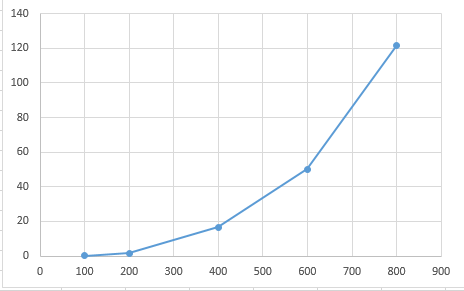
\includegraphics{genetic}

Zakładając stałą liczbę iteracji głównej pętli na złożoność składają się:

\begin{itemize}
\item Krzyżowanie - pętla wykonywająca się tak długo aż dziecko będzie miało wszystkie oligonukleotydy rodziców - liczba oligo w spektrum jest zależna od n - długości dna, a także od temperatury. Wszystkie kroki w pętli mają czas stały lub zależny liniowo od n np. znalezienie elementu w spektrum - a więc ogólna złożoność funkcji jest kwadratowa.

\item Mutacje - liczba mutacji jest uzależniona od rozmiaru spektrum - złożoność liniowa. Wszystkie operacje występujące w funkcji mutacji również
mają koszt liniowy np. koszt znalezienia najgorszego elementu. Również i tutaj ogólna złożoność jest zależna od kwadratu z n.
           
\item Losowanie początkowej populacji, generowanie chwilowego rozwiązania mają złożoność liniową.

\item Wybranie najlepszych rodziców czyli de facto posortowanie całej populacji ma złożoność n*log(n) - stosujemy sortowanie szybkie - quicksort z biblioteki algorithm.
\end{itemize}

Co ciekawe wraz ze zwiększaniem temperatury rośnie, rośnie również czas wykonywania algorytmu co jest spowodowane trudniejszym dopasowywaniem oligonukleotydów do siebie - duży narzut ma tutaj krzyżowanie rodziców.

\section{Algorytm dokładny}

Algorytm ten okazał się typowym problemem grafowym - co ciekawe, mającym wiele wspólnego z znanym powszechnie \textit{problemem komiwojażera}. W związku z tym opracowanie oraz implementacja algorytmu dokładnego nie należało do wybitnie wymagających zadań w tym projekcie, gdyż podobne problemy rozwiązywaliśmy już w poprzednich latach studiów (nie mówiąc już o ogromie literatury traktującej o tego typu problemach).

Kluczową elementem tego algorytmu było wyznaczanie \textit{overlapu}, czyli długości części wspólnej dwóch dowolnych nukleotydów dostępnych w spektrum. Na podstawie tej informacji tworzyliśmy odpowiednie połączenia między dwoma nukleotydami w grafie.

Po wygenerowaniu grafu problem sprowadzał się do wyszukania optymalnej ścieżki za pomocą algorytmu przechodzenia grafu w głąb.

\subsection{Opis}

Nasze rozwiązanie dzieli się na dwa etapy: generowania grafu na podstawie spektrum oraz poszukiwanie optymalnej sekwencji nukleotydów za pomocą przeszukiwania grafu.

Na początku pierwszego etapu każdy element spektrum dodajemy do listy wierzchołków. Każdy wierzchołek zawiera wartość nukleotydu, ilość powtórzeń w spektrum oraz listę krawędzi, które wychodzą z danego wierzchołka (domyślnie jest ona pusta). Dla uproszczenia założyliśmy, że w przypadku wielokrotnego występowania danego nukleotydu nie będziemy dodawać nowego wierzchołka do grafu, a jedynie zwiększymy licznik wystąpień w wierzchołku już istniejącym. 

Następnie spośród wszystkich elementów dostępnych w spektrum generujemy pary. Dla każdej z nich uruchamiamy procedurę wyliczającą \textit{overlap} między nimi. Jeżeli istnieje jakikolwiek część wspólna między nimi, do wierzchołka źródłowego dodajemy krawędź o wadze równej wyliczonego \textit{overlapu} oraz danym wierzchołkiem docelowym. 

Drugi etap stanowi zmodyfikowaną odmianę algorytmu \textit{DFS}. Początkowo na stosie ustawiamy wierzchołek początkowy (czyli znany nam pierwszy nukleotyd w sekwencji DNA), a następnie rekurencyjnie przechodzimy po wszystkich jego sąsiadach. Fakt odwiedzin danego wierzchołka oznaczamy w tablicy \textit{visited} będącym słownikiem, którego kluczem jest wskaźnik do wierzchołka, a wartością ilość powtórzeń danego nukleotydu w spektrum. W przypadku odwiedzin dekrementujemy licznik - jeżeli osiągnie on wartość zero, uznajemy wierzchołek za już odwiedzony. 

Algorytm przeszukiwania potrafi zwrócić więcej niż jedną ścieżkę - dlatego też za każdym razem  sprawdzamy, czy wygenerowana ścieżka zawiera wszystkie oligonukleotydy dostępne w spektrum. W przypadku znalezienia takiej ścieżki, o ile wcześniej nie została znaleziona ścieżka o krótszej trasie, zostaje ona zapisana w specjalnej zmiennej. Po zakończeniu przeszukiwania w tej zmiennej będzie znajdowała się końcowa sekwencja DNA.

\subsection{Złożoność}

W tym algorytmie nie jest problemem wygenerowanie odpowiedniego grafu - kluczem jest w tym przypadku proces przeszukiwania grafu, który \textit{de facto} jest zmodyfikowaną odmianą poszukiwania ścieżki Hamiltona. Problem ten należy do grupy silnie NP-trudnych, co oznacza, że możemy nie doczekać się wyniku w rozsądnym czasie. 

Dlatego też powyższy algorytm bardzo dobrze radzi sobie z mniejszymi instancjami, w przypadku których czas realizacji tego algorytmu należy jeszcze do "akceptowalnych". W przypadku większych spektrum pozostaje już tylko wyłącznie korzystanie z algorytmów przybliżonych.

\section{Testy}

\subsection{Algorytm przybliżony}

\begin{longtable}{c|c|c|c|c}
Długość  & Temperatura  & Błąd & Czas    & Wynik  \\
\hline
100    & 20   & 0     & 0,24    & 85    \\
100    & 20   & 0,05  & 0,23    & 86    \\
100    & 20   & 0,1   & 0,25    & 85    \\
100    & 20   & 0,15  & 0,22    & 88    \\
100    & 20   & 0,2   & 0,24    & 83    \\
100    & 20   & 0,3   & 0,25    & 86    \\
100    & 30   & 0     & 0,26    & 73    \\
100    & 30   & 0,05  & 0,26    & 75    \\
100    & 30   & 0,1   & 0,26    & 73    \\
100    & 30   & 0,15  & 0,25    & 75    \\
100    & 30   & 0,2   & 0,25    & 68    \\
100    & 30   & 0,3   & 0,27    & 67    \\
100    & 40   & 0     & 0,29    & 69    \\
100    & 40   & 0,05  & 0,29    & 76    \\
100    & 40   & 0,1   & 0,29    & 76    \\
100    & 40   & 0,15  & 0,28    & 72    \\
100    & 40   & 0,2   & 0,29    & 68    \\
100    & 40   & 0,3   & 0,29    & 65    \\
100    & 50   & 0     & 0,62    & 78    \\
100    & 50   & 0,05  & 0,58    & 72    \\
100    & 50   & 0,1   & 0,59    & 70    \\
100    & 50   & 0,15  & 0,63    & 67    \\
100    & 50   & 0,2   & 0,6     & 69    \\
100    & 50   & 0,3   & 0,6     & 69    \\
200    & 20   & 0     & 1,57    & 86    \\
200    & 20   & 0,05  & 1,57    & 80    \\
200    & 20   & 0,1   & 1,55    & 75    \\
200    & 20   & 0,15  & 1,58    & 78    \\
200    & 20   & 0,2   & 1,57    & 67    \\
200    & 20   & 0,3   & 1,53    & 63    \\
200    & 30   & 0     & 2       & 79    \\
200    & 30   & 0,05  & 1,92    & 78    \\
200    & 30   & 0,1   & 1,93    & 80    \\
200    & 30   & 0,15  & 1,9     & 78    \\
200    & 30   & 0,2   & 1,92    & 72    \\
200    & 30   & 0,3   & 1,92    & 60    \\
200    & 40   & 0     & 2,34    & 73    \\
200    & 40   & 0,05  & 2,29    & 79    \\
200    & 40   & 0,1   & 2,3     & 70    \\
200    & 40   & 0,15  & 2,26    & 70    \\
200    & 40   & 0,2   & 2,32    & 66    \\
200    & 40   & 0,3   & 2,25    & 59    \\
200    & 50   & 0     & 4,86    & 77    \\
200    & 50   & 0,05  & 4,7     & 74    \\
200    & 50   & 0,1   & 4,5     & 78    \\
200    & 50   & 0,15  & 4,77    & 76    \\
200    & 50   & 0,2   & 4,71    & 70    \\
200    & 50   & 0,3   & 4,82    & 58    \\
400    & 20   & 0     & 16,61   & 78    \\
400    & 20   & 0,05  & 16,07   & 70    \\
400    & 20   & 0,1   & 15,66   & 69    \\
400    & 20   & 0,15  & 16,1    & 69    \\
400    & 20   & 0,2   & 16,15   & 69    \\
400    & 20   & 0,3   & 15,71   & 60    \\
400    & 30   & 0     & 17,52   & 75    \\
400    & 30   & 0,05  & 17,39   & 75    \\
400    & 30   & 0,1   & 17,64   & 74    \\
400    & 30   & 0,15  & 17,67   & 73    \\
400    & 30   & 0,2   & 18,47   & 72    \\
400    & 30   & 0,3   & 18,32   & 73    \\
400    & 40   & 0     & 27      & 79    \\
400    & 40   & 0,05  & 26,77   & 80    \\
400    & 40   & 0,1   & 27,02   & 73    \\
400    & 40   & 0,15  & 27,08   & 71    \\
400    & 40   & 0,2   & 26,4    & 73    \\
400    & 40   & 0,3   & 26,7    & 67    \\
400    & 50   & 0     & 45,58   & 83    \\
400    & 50   & 0,05  & 45,35   & 87    \\
400    & 50   & 0,1   & 45,22   & 82    \\
400    & 50   & 0,15  & 44,5    & 91    \\
400    & 50   & 0,2   & 43,68   & 89    \\
400    & 50   & 0,3   & 44,6    & 81    \\
600    & 20   & 0     & 50,25   & 77    \\
600    & 20   & 0,05  & 49,62   & 76    \\
600    & 20   & 0,1   & 51,19   & 75    \\
600    & 20   & 0,15  & 51,88   & 72    \\
600    & 20   & 0,2   & 51,06   & 72    \\
600    & 20   & 0,3   & 50,28   & 70    \\
600    & 30   & 0     & 55,56   & 82    \\
600    & 30   & 0,05  & 55,39   & 80    \\
600    & 30   & 0,1   & 55,42   & 79    \\
600    & 30   & 0,15  & 55,65   & 74    \\
600    & 30   & 0,2   & 54,01   & 75    \\
600    & 30   & 0,3   & 55,48   & 60    \\
600    & 40   & 0     & 81,54   & 86    \\
600    & 40   & 0,05  & 84,4    & 79    \\
600    & 40   & 0,1   & 81,95   & 76    \\
600    & 40   & 0,15  & 85,4    & 74    \\
600    & 40   & 0,2   & 85,25   & 74    \\
600    & 40   & 0,3   & 84,22   & 69    \\
600    & 50   & 0     & 141,99  & 80    \\
600    & 50   & 0,05  & 154,01  & 78    \\
600    & 50   & 0,1   & 138,83  & 77    \\
600    & 50   & 0,15  & 139,44  & 72    \\
600    & 50   & 0,2   & 134,96  & 70    \\
600    & 50   & 0,3   & 137,53  & 65    \\
800    & 20   & 0     & 121,74  & 80    \\
800    & 20   & 0,05  & 121,26  & 79    \\
800    & 20   & 0,1   & 119,8   & 76    \\
800    & 20   & 0,15  & 118,82  & 76    \\
800    & 20   & 0,2   & 118,88  & 75    \\
800    & 20   & 0,3   & 118,34  & 59    \\
800    & 30   & 0     & 126,76  & 76    \\
800    & 30   & 0,05  & 127,12  & 76    \\
800    & 30   & 0,1   & 124,98  & 75    \\
800    & 30   & 0,15  & 127,04  & 73    \\
800    & 30   & 0,2   & 126,84  & 76    \\
800    & 30   & 0,3   & 126,79  & 75    \\
800    & 40   & 0     & 189,99  & 73    \\
800    & 40   & 0,05  & 190,59  & 73    \\
800    & 40   & 0,1   & 190,17  & 69    \\
800    & 40   & 0,15  & 189,66  & 68    \\
800    & 40   & 0,2   & 189,67  & 70    \\
800    & 40   & 0,3   & 190,09  & 83    \\
800    & 50   & 0     & 321,19  & 76    \\
800    & 50   & 0,05  & 321,34  & 78    \\
800    & 50   & 0,1   & 319,57  & 79    \\
800    & 50   & 0,15  & 322,12  & 76    \\
800    & 50   & 0,2   & 320,97  & 77    \\
800    & 50   & 0,3   & 317,73  & 65    \\
1600   & 20   & 0     & 921,13  & 68    \\
1600   & 20   & 0,05  & 951,33  & 66    \\
1600   & 20   & 0,1   & 921,33  & 65    \\
1600   & 20   & 0,15  & 921,23  & 67    \\
1600   & 20   & 0,2   & 1031,93 & 55    \\
1600   & 20   & 0,3   & 1221,33 & 55    \\
1600   & 30   & 0     & 1221,52 & 65    \\
1600   & 30   & 0,05  & 1261,34 & 64    \\
1600   & 30   & 0,1   & 1271,21 & 63    \\
1600   & 30   & 0,15  & 1255,65 & 60    \\
1600   & 30   & 0,2   & 1266,44 & 66    \\
1600   & 30   & 0,3   & 1366,74 & 55    \\
1600   & 40   & 0     & 1601,23 & 62    \\
1600   & 40   & 0,05  & 1602,43 & 61    \\
1600   & 40   & 0,1   & 1640,89 & 60    \\
1600   & 40   & 0,15  & 1649,12 & 59    \\
1600   & 40   & 0,2   & 1602,21 & 58    \\
1600   & 40   & 0,3   & 1690,32 & 58    \\
1600   & 50   & 0     & 2144,34 & 66    \\
1600   & 50   & 0,05  & 2137,14 & 66    \\
1600   & 50   & 0,1   & 2140,88 & 64    \\
1600   & 50   & 0,15  & 2212,23 & 63    \\
1600   & 50   & 0,2   & 2190,12 & 58    \\
1600   & 50   & 0,3   & 2200,93 & 55   
\end{longtable}

Efektywność algorytmu pomału maleje dla długich łańcuchów - jasne jest że trudniej skonstruować poprawny długi łańcuch. Oś y reprezentuje procent zgodności z oryginalną sentencją, a oś x długość odcinka DNA:


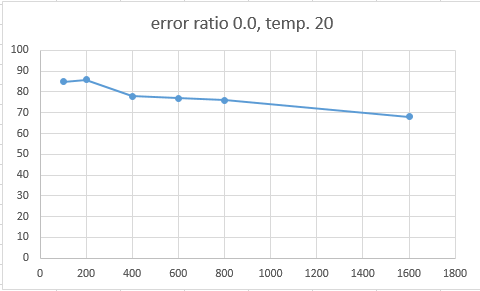
\includegraphics{temp20err000}

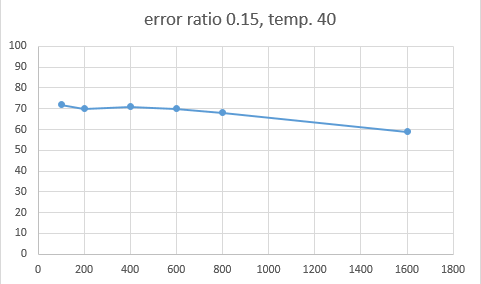
\includegraphics{temp40err015}

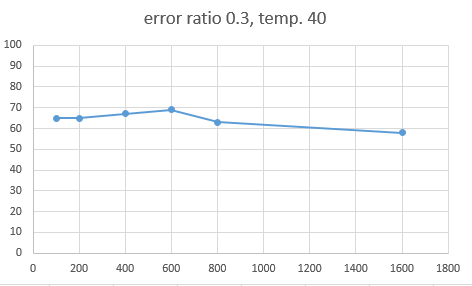
\includegraphics{temp40err030}

Poniższe wykresy obrazują wielomianową złożoność algorytmu, udaje nam się osiągać rozsądne czasy nawet dla dużych wielkości instancji. Oś y reprezentuje czas wyrażony w sekundach, a oś x długość odcinka DNA:

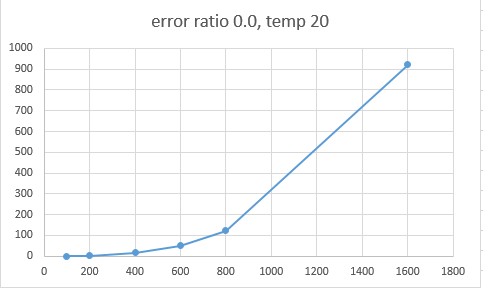
\includegraphics{temp20err000time}

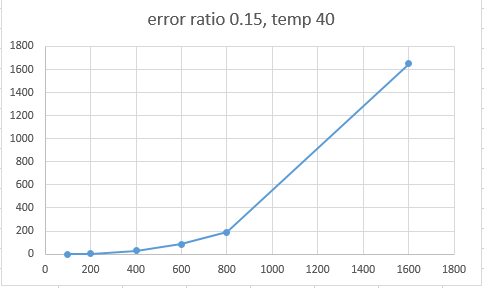
\includegraphics{temp40err015time}

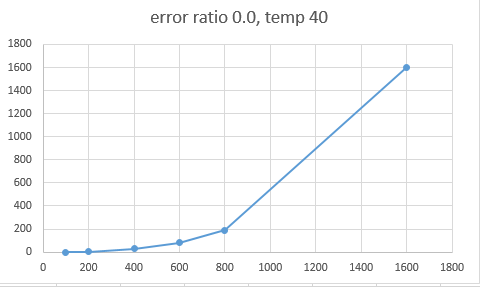
\includegraphics{temp40err000time}

\subsection{Algorytm dokładny}

\begin{longtable}{c|c|c|c|c}
Długość  & Temperatura  & Błąd & Czas  \\
\hline
10     & 20   & 0     & 0,01   \\
10     & 20   & 0.5   & 0,01   \\
10     & 20   & 0.1   & 0,01   \\
10     & 20   & 0.15  & 0,01   \\
10     & 30   & 0     & 0,00   \\
10     & 30   & 0.5   & 0,00   \\
10     & 30   & 0.1   & 0,00   \\
10     & 30   & 0.15  & 0,00   \\
10     & 40   & 0     & 0,00   \\
10     & 40   & 0.5   & 0,00   \\
10     & 40   & 0.1   & 0,00   \\
10     & 40   & 0.15  & 0,00   \\
15     & 20   & 0     & 0,98   \\
15     & 20   & 0.5   & 0,97   \\
15     & 20   & 0.1   & 0,96   \\
15     & 20   & 0.15  & 0,97   \\
15     & 30   & 0     & 0,04   \\
15     & 30   & 0.5   & 0,05   \\
15     & 30   & 0.1   & 0,04   \\
15     & 30   & 0.15  & 0,04   \\
15     & 40   & 0     & 0,00   \\
15     & 40   & 0.5   & 0,00   \\
15     & 40   & 0.1   & 0,00   \\
15     & 40   & 0.15  & 0,00   \\
20     & 20   & 0     & 102,46 \\
20     & 20   & 0.5   & 102,73 \\
20     & 20   & 0.1   & 104,52 \\
20     & 20   & 0.15  & 103,51 \\
20     & 30   & 0     & 3,30   \\
20     & 30   & 0.5   & 3,09   \\
20     & 30   & 0.1   & 3,12   \\
20     & 30   & 0.15  & 3,06   \\
20     & 40   & 0     & 0,06   \\
20     & 40   & 0.5   & 0,06   \\
20     & 40   & 0.1   & 0,06   \\
20     & 40   & 0.15  & 0,06   \\
25     & 20   & 0     & 915,12 \\
25     & 20   & 0.5   & 912,87 \\
25     & 20   & 0.1   & 918,47 \\
25     & 20   & 0.15  & 911,42 \\
25     & 30   & 0     & 140,24 \\
25     & 30   & 0.5   & 140,88 \\
25     & 30   & 0.1   & 140,10 \\
25     & 30   & 0.15  & 140,19 \\
25     & 40   & 0     & 28,44  \\
25     & 40   & 0.5   & 29,00  \\
25     & 40   & 0.1   & 28,01  \\
25     & 40   & 0.15  & 28,36 
\end{longtable}


\section{Podsumowanie}

...

\end{document}

